\documentclass{article}

\usepackage[utf8]{inputenc}
\usepackage[english]{babel}
\usepackage{dsfont}
\usepackage{amsmath}
\usepackage{ mathrsfs }
\usepackage{amssymb}
\usepackage{graphicx}% Include figure files
\usepackage{dcolumn}% Align table columns on decimal point
\usepackage{bm}% bold math
\usepackage{amsmath}
\usepackage{varioref}
\usepackage{booktabs}
\usepackage[bottom]{footmisc}
\usepackage{csvsimple}

\usepackage{algpseudocode}
\usepackage{listings}

\usepackage{lmodern}
\usepackage{tikz}
\usepackage{kantlipsum}
\usetikzlibrary{calc,patterns,angles,quotes}

\newcommand{\RN}[1]{%
  \textup{\uppercase\expandafter{\romannumeral#1}}%
}




\usepackage[utf8]{inputenc}

\usepackage{natbib}
\usepackage{graphicx}
\usepackage[]{hyperref}
\usepackage[]{physics}
\usepackage[]{listings}
\usepackage[T1]{fontenc}
\usepackage{color}
\usepackage{float}
\usepackage{soul}
\lstset{
  backgroundcolor=\color{white}, % requires \usepackage{color} or \usepackage{xcolor}
  basicstyle=\footnotesize,
  breakatwhitespace=false,
  breaklines=true,
  captionpos=b,
  commentstyle=\color{green},
  deletekeywords={...},
  escapeinside={\%*}{*)},
  extendedchars=true,
  frame=single,
  keepspaces=true,
  keywordstyle=\color{blue},
  language=c++,
  otherkeywords={*,...},
  rulecolor=\color{black},
  showspaces=false,
  showstringspaces=false,
  showtabs=false,
  stepnumber=2,
  %stringstyle=\color{pink},
  tabsize=4,
}

\title{Numerical integration}
\author{
  Brandt, Samuel\\
 % \texttt{}
  \and
  Davidov, Aleksandar\\
  \textcolor{blue}{\href{https://github.com/aleksda/FYS4150/}{\texttt{github.com/aleksda}}}
  \and
  Hemaz, Said\\
  % \texttt{first2.last2@xxxxx.com}
}
\date{October 2019}



\begin{document}

\maketitle




\section{Abstract}
The purpose of this project is to find the expectation value of the quantum mechanical correlation energy between two electrons in the helium atom. Four different methods was used to approximate the answer. This are Gauss-Legendre, Gauss-Laguerre, Monte Carlo with brute-force , Monte Carlo with sampling and finally the last mentioned code with parallization applied. The last method proved to be superior as it calculated good results within a matter of seconds , where for instance the Gauss-Legendre gives unsatisfactory results at undesirable slow speed. The most accurate method in our experiment was Gauss-Laguerre although it also was the most time consuming in terms of speed.\\\\\\\\\\\\\\\\\\\\\\\\\\\\\\\\\\\\\\\\

\tableofcontents

\newpage

\iffalse
\begin{figure}[h!]
\centering
\includegraphics[scale=3.0]{universe}
\caption{The Universe}
\label{fig:universe}
\end{figure}
\fi
\newpage
\section{Introduction}

Integrals are one of the main mathematical tools we use to describe many phenomena in science. Even though many of them can be solved analytically for a precise answer, a great deal of them can not. This brings us to the numerical methods, which gives us another challenge, round off errors. For our project, we utilize the Gaussian quadrature with weight functions based on Legendre and Laguerre polynomials, as well as three Monte Carlo methods to solve a quantum mechanical integral, specifically the quantum mechanical expectation value of the correlation energy between two electrons.


\section{Theory}

We make the assumption that the wave function of each electron can be written as a single-particle wave function for an electron in a hydrogen atom. The single-particle wave function is given as :
\[
   \psi_{1s}({\bf r}_i)  =   e^{-\alpha r_i},
\]
\ Where the wave position vector ${\bf r}_i$, is:\\ 
\[
   {\bf r}_i =  x_i {\bf e}_x + y_i {\bf e}_y +z_i {\bf e}_z ,
\]
and the magnitude  ${ r}_i$ is given as:

\[
r_i = \sqrt{x_i^2+y_i^2+z_i^2}.
\]
The total wave-function for both electrons can be written as:
\[
   \Psi({\bf r}_1,{\bf r}_2)  =   e^{-\alpha (r_1+r_2)}.
\]
The equation above is not normalized, but this has been deemed to be irrelevant and it will not be taken under consideration by this project. \

We place $\alpha=2$, which represents the charge for the helium atom $Z=2$.
The integral we are going to solve , will be the expectation value of quantum mechanical correlation energy between to electrons in the helium atom that repulses each other through a Coulomb-potential is:

\begin{equation}\label{eq:correlationenergy}
   \langle \frac{1}{|{\bf r}_1-{\bf r}_2|} \rangle =
   \int_{-\infty}^{\infty} d{\bf r}_1d{\bf r}_2  e^{-2\alpha (r_1+r_2)}\frac{1}{|{\bf r}_1-{\bf r}_2|}.
\end{equation}

This integral has the exact solution of  $5\pi^2/16^2$.  Later in this project we will be approximating this answer through four different methods. \\


Numerically, the integration limits will be $\pm \infty$ , this is hard to implement. An easier way to rewrite this will be to change the variables to spherical coordinates, in this case we transform 4 out of six infinite integrals.
the volume elements in spherical coordinates can be written as
\begin{align}
	\d\mathbf{r}_i = r_i^2\sin (\theta_i)\d \theta_i \d \phi_i \d r_i
\end{align}
where $r_i \in [0, \infty)$, $\theta_i \in [0, \pi]$ and $\phi_i \in [0, 2\pi]$. The magnitude of the distance between the electrons is 
\begin{align}
	|\mathbf{r}_1 - \mathbf{r}_2| = r_{12} = \sqrt{r_1^2 + r_2^2 - 2r_1 r_2 \cos \beta}
\end{align}
where
\begin{align}
	\cos\beta = \cos(\theta_1) \cos (\theta_2) + \sin(\theta_1)\sin(\theta_2) \cos(\phi_1 - \phi_2) \nonumber
\end{align}
The integral in spherical coordinates is then
\begin{align}
	\langle \frac{1}{r_{12}} \rangle = \int \d r_1 \d r_2 \d \theta_1 \d \theta_2 \d \phi_1 \d \phi_2 \frac{1}{r_{12}} r_1^2r_2^2\sin(\theta_1)\sin(\theta_2) e^{-2\alpha(r_1+r_2)}
\end{align}


\section{Methods}

\subsection{Gaussian quadrature}\label{const_mot}

The idea behind Gaussian quadrature is to approximate the integral of a function $f$ by
\begin{align}
	I = \int_{a}^{b} f(x) \ \d x  = \int_{a}^{b} W(x)g(x) \ \d x \approx \sum_{i=1}^N w_i g(x_i) 
\end{align}

where $W(x)$ is a weight function that can be derived through a polynomial which is orthogonal in the interval $[a, b]$. Example of such weighted functions are $W(x)=1$ (Legendre polynomials in the interval $x\in[-1, 1]$) and and $W(x) = x^\alpha e^{-x}$ (Laguerre polynomials in the interval $x \in [0, \infty)$). 

\subsection{Gauss-Legendre}\label{const_mot}

The polynomials of Gauss-Legendre are defined on the interval $[-1, 1]$ with a weight
function $W(x) = 1$.  through change of variables , we could choose another interval than $[-1, 1]$. The numerical accuracy is However, one must note that this can significantly
degrade the numerical accuracy. The Gauss-Legendre quadrature gives rise to the following
relation:

\begin{align*}
  I = \int_{-1}^{1} f(x) \, dx = \int_{-1}^{1}W(x)g(x)\, dx = \int_{-1}^{1}g(x)
  \, dx = \sum^{N}_{i=1} \omega_ig(x_i)
\end{align*}
It turns out that the associated integration points $x_i$ are the roots of the
Legendre polynomials. We can rewrite this integral in the Legendre form using a simple change of variables.
\\
When working with cartesian co-ordinates we get a six dimensional integral which is why our Gauss-Legendre function uses six for-loops for each desired n . This gives the function a big-O notation of $O(n^6)$ and is the reason for the slow moving pace of this function. 

\subsection{Gauss-Laguerre}\label{const_mot}
The  polynomials of Gauss-Laguerre are orthogonal on $[0, \infty)$ and have a
weight function $W(x) = x^\alpha e^{-x}$. These properties, gives us the relation:\\

\begin{align}
  \notag I = \int_0^\infty f(x) \, dx = \int_0^\infty W(x)g(x) \, dx =
  \int_0^\infty x^\alpha e^{-x} g(x) \, dx = \sum^{N}_{i=1} \omega_ig(x_i)
\end{align}

In order to use the Gauss-Laguerre quadrature, we need to modify eq. (1)
to spherical coordinates. 
\begin{align*}
  I &= \int_{-\infty}^{\infty} d\v{r}_1d\v{r}_2 e^{-4(r_1, r_2)} \frac{1}{\left| \v{r}_1 - \v{r}_2 \right|}.\\
    &= \intlimits r_1^2r_2^2e^{-4r_1} e^{-4r_2} \gamma(\beta)\sin\theta_1\sin\theta_2 dr_1dr_2d\theta_1d\theta_2d\phi_1d\phi_2\\
  \intertext{Substituting $u_i = 4r_i$, $i = 1, 2$ yields}
  &= \frac{1}{1024}\intlimits u_1^2u_2^2e^{-u_1}e^{-u_2} \frac{\sin\theta_1\sin\theta_2}{\sqrt{u_1^2 + u_2^2 - 2u_1r_2\cos\beta}} du_1du_2d\theta_1d\theta_2d\phi_1d\phi_2\\
    &=\frac{1}{1024} \int_{0}^\infty\int_0^\infty\int_0^{\pi}\int_0^\pi\int_0^{2\pi}\int_0^{2\pi}W(u_1)W(u_2)g(u, \theta, \phi)\,du_1du_2d\theta_1d\theta_2d\phi_1d\phi_2.
\end{align*}

Based on these limits it can be practical to apply Gauss-Laguerre  for
the two initial integrals, and use Gauss-Legendre for the remaining four.
Since we still use a six-dimensional integral the big-O notation remains $O(n^6)$.\\\

The function call in the code looked something like this in C++:
\begin{lstlisting}
    gauss_laguerre(x_r, weight_r, steps, alfa);
    gauleg(angle_start, angle_end, x_theta, weight_theta, steps);
    gauleg(angle_start, 2*angle_end, x_phi, weight_phi, steps);
\end{lstlisting}

Where gauleg() is a function you can find in the 'lib.cpp' library

\begin{figure}[H]
    \centering
	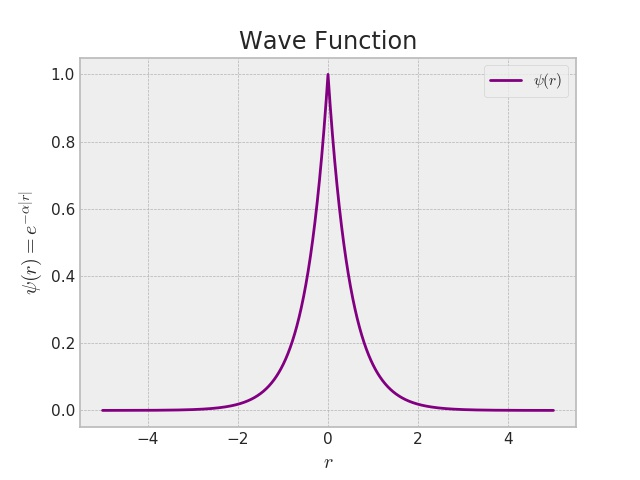
\includegraphics[scale=0.4, clip=true, trim= 0 0 0 0]{wave_func.jpg}
	\caption{Plot of $e^{-\alpha |x|}$ to find appropriate integration limits for Gauss-Legendre quadrature. We see that the function is more or less zero for $x\approx \pm3$.}
	\label{fig: integration limits Gauss-Legendre}
\end{figure} 


\subsection{Monte Carlo (MC) }\label{const_mot}
Monte Carlo integration is an inherently non-deterministic algorithm, meaning there is always an error related to the random aspect of the calculations. Here we sample points randomly, computing only the integral itself will not be enough, therefore we have to also compute the standard deviation or the variance, to get a view of the uncertainty in the results. We begin with sampling point and picking numbers at random in a the interval $[0, 1]$, this approach is also known as the "brute force" method. Another method is to simply find a probability density function (PDF) using MC- importance sampling , that resembles the function that we want to integrate.


\subsubsection{Brute-force Monte Carlo}
\label{sub:brute_force_monte_carlo}

The PDF associated with the MC- brute force method is
the uniform distribution given by
\begin{equation}
  \notag
  p(x) = \begin{cases}
    \frac{1}{b-a}, & x \in [a, b] \\
    0, & x \in [a, b]^{\complement}.
  \end{cases}
\end{equation}
Here, $a,b \in \mathbb{R}$, and the lower case 'C' denotes the complement of the set.
Since $p(x)$ results in  $\int_{-\infty}^\infty p(x) \, dx = 1$ we have that
\begin{align*}
  \notag
  \langle f \rangle = \int_{-\infty}^\infty p(x) f(x) \, dx = \int_0^1 p(x)f(x) \, dx &\approx \sum^{N}_{i=1} f(x_i).
\end{align*}
For more general use of integration limits $a, b$ , applying the fact that the conservation of probability is  $p(y)dy = dx$, then the standard change
of variables will be sufficient for : $y(x) = a + (b - a)x$.\\\

\subsubsection{Monte Carlo with important sampling}\label{const_mot}

In this version of MC we need to find a PDF  $p(y)$ that mimics  $f(x)$ of the chosen integration interval.  In this case it is fitting to use  $p(y) = e^{-y}$ as the exponential distribution, yielding $p(r) = e^{-4r}$ with the normalization requirement :

\begin{equation}
  \notag
  p(r) = Ae^{-4r}
\end{equation} 

which is the PDF. We change the integral to spherical coordinates so that we can apply this PDF.

In order to make this work for any given interval, we implement the change of variable
\begin{equation}
  \notag
  y(x) = -\frac{\ln(1 - x)}{2\alpha}
\end{equation}
which yields the values for $y \in [0, \infty)$.

\subsubsection{Monte Carlo with important sampling with parallization}\label{const_mot}
In order to further optimize our results with MC-method , it is ideal to have N (sample points) as big as possible. To achieve this we use use different compiler flags, and parallization with OpenMP.
\\
The C++ implementation of the parallized MC-algorithm is as follows:
\begin{lstlisting}
#pragma omp parallel for reduction(+:cmc, sigma) private(i)
    for(i = 0; i < n; i++) {

        u 	= -log(1.-ran());
        v 	= -log(1.-ran());
        theta1 	= M_PI * ran();
        theta2 	= M_PI * ran();
        phi1 	= 2 * M_PI * ran();
        phi2 	= 2 * M_PI * ran();

        func = integrate(u, v, theta1, theta2, phi1, phi2);

        cmc   += func;
        sigma += func * func;

    } 

\end{lstlisting}

Note, that in order to parallize our program we use the decorator #\textit{pragma} on the first line.

\section{Results/Analysis}¨
	\subsection{Gauss Quadrature}
	
	    Table 1 \& 2 shows the two Gauss Quadrature methods compared in terms of errors and CPU time. The results for the Gaussian Legendre converge at a level of three digits at around 10 mesh points. We can see that the error on the Legendre method is higher than the Laguerre method, also the time is slower in terms of the non-satisfactory results that it produced compared to Laguerre. For N = 40 it takes around 400 seconds , with a relative error of around 2,5 \%, it might seem like not much but in many cases is not good enough. The results on Laguerre shows that even after the N = 15 mark, it only takes around 2 seconds , for a better result than the Gauss Legendre method. It is then concluded that the Gauss Laguerre method comes out on top compared to Gauss Legendre, even if it uses a bit more time. 

		\begin{table}[h]
			\centering
			\caption{Results from a run of the program which calculates the integral using Gauss- Quadrature methods in terms of error. Exact value is 0.192766.}
			\label{table: Error results Gauss-Quarature}
			\begin{tabular}{|c|c|c|}
\hline
\textbf{N} 	&	\textbf{Gauss- Legendre}	&	\textbf{Gauss- Laguerre} \\\hline 
10 	&	0.0707	&	0.004759					\\ \hline
15 	&	0.040	&	0.002887				\\ \hline
20 	&	0.0298	&	0.002526			\\ \hline
30 	&	0.0255	&	0.002044				\\ \hline
40 	&	0.0247	&	0.001811					\\ \hline
			\end{tabular}
		\end{table}
And the second table, 
		\begin{table}[h]
			\centering
			\caption{Results from a run of the program which calculates the integral using the Gauss- Quadrature methods in terms of CPU time . Exact value is 0.192766.}
			\label{table: Error results Gauss-Quarature}
			\begin{tabular}{|c|c|c|}
\hline
\textbf{N} 	&	\textbf{Gauss- Legendre}	&	\textbf{Gauss- Laguerre} \\\hline 
10 	&	0.195 s	& 0.328072 s					\\ \hline
15 	&	1.35 s	& 2.0626 s 					\\ \hline
20 	&	7.46 s	& 12.6147 s					\\ \hline
30 	&	83.3 s	& 117.602 s						\\ \hline
40 	&	473 s	& 612.977 s						\\ \hline

			\end{tabular}
		\end{table}


	
	\subsection{MC methods}
        
        Now, the tables for the MC methods. As we see in table 3 and 4, the results in general gets better as the number N increases. We can also see a considerable difference between the MC methods compared to Gauss- Quadrature methods in terms of CPU speed. \\
        
        If we make the comparison between the MC methods we can clearly see the the MC importance sampling methods produces the best results in terms of accuracy due to the very low error value. This is especially true for the parallized version of the MC importance sampling, with the use of two processors with two threads each.   Even at sampling point N = $10^5$ we get better results than any of the other methods.  \\
        
        The variance also got a greater value going from MC brute force to MC- importance sampling, most likely because it gets closer to the analytical variance. In relation to the time , the fastest method however was the MC  brute force even though it produces less accurate results, if we leave parallization out of the picture. With parallization, we clearly see in the results that the MC importance sampling method is the fastest and most accurate. \\

		\begin{table}[h]
			\centering
			\caption{Results from a test of the program which calculates the integral using the Monte Carlo methods. The errors are averaged over 6 runs of the program. The exact value of the integral is 0.192766.}
			\label{table: results brute force MC}
			\begin{tabular}{|c|c|c|c|}
\hline
\textbf{N} 	&	\textbf{MC -BF}	&	\textbf{MC - IS }	&	\textbf{MC - IS with Parallization} \\ \hline 
10^4 	&	0.184	&	0.0111			&	0.0525	\\ \hline
10^5 	&	0.133	&	0.01			&	0.00485	\\ \hline
.. 	&	...	&	...			&	...	                \\ \hline
10^8 	&	0.0384	&	0.0000491			&	0.00134 	\\ \hline
10^9 	&	0.0019	&	0.0000234		&	0.000516	\\ \hline
			\end{tabular}
		\end{table}
Now, table (4) will give us an comparison of the CPU-time for each method.

		\begin{table}[h]
			\centering
			\caption{Results from a run of the program which calculates the integral using the Monte Carlo methods. The CPU-time are averaged over 6 runs of the program. The exact value of the integral is 0.192766.}
			\label{table: results brute force MC}
			\begin{tabular}{|c|c|c|c|}
\hline
\textbf{N} 	&	\textbf{MC -BF}	&	\textbf{MC - IS }	&	\textbf{MC - IS with Parallization} \\ \hline 
10^4 	&	0.00122 s	&	0.000874 s			&	$0.000394 $ s	\\ \hline
10^5 	&	0.00712 s	&	0.00993 s			&	$0.00162 $s	\\ \hline
.. 	&	...	&	...			&	...	                \\ \hline
10^8 	&	2.94 s	&	4.95 s			&	$0.107 $ s	\\ \hline
10^9 	&	24.3 s	&	45.3 s			&	$1.42 $ s	\\ \hline
			\end{tabular}
		\end{table}\\\\\\\\\

\newpage

We also compared the error of the codes with compiler flags,  such as the \textit{O2} and \textit{O3} flags.Figure \cite{fig: WHAT} shows the comparison between the parallel Monte Carlo algorithm with the O2 and O3 compiler flags. As we can see the compiler flags helped to drastically reduce the error. Already after $n=10^5$ iterations we see that the the compiler flags got results very close to the analytical one. While the one without flags reached it's peak at around $n=10^7$ iterations. \\

\begin{figure}[H]
	\centering
	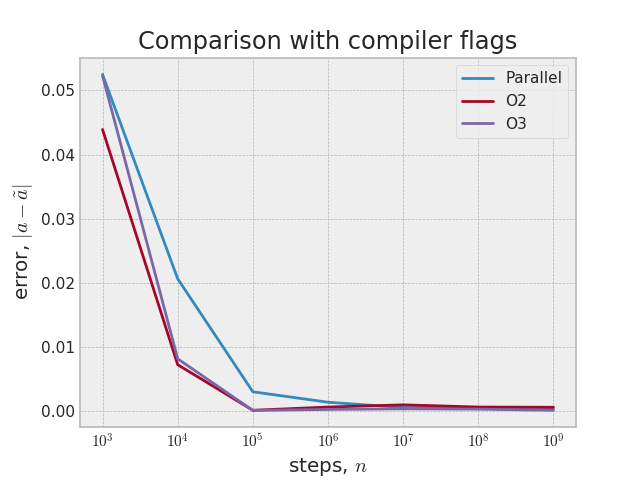
\includegraphics[scale=0.5, clip=false, trim= 0 0 0 0]{compiler_flags.png}
	\caption{Plot that compares the compiler flags used on the parallization of MC importance sampling.}
	\label{fig: integration limits Gauss-Legendre}
\end{figure}



\section{Conclusion}

In this project we have shown that certain modifications of an integral can give us huge simplifications in terms of numerical integration. Gaussian quadrature Laguerre proves to be superior to Gaussian Quadrature Legendre, in terms general accuracy but have about the same degree of time-usage due to the fact that they both share the same big-O notation of $O(n^6)$ .  
If we look at the Monte Carlo methods, they are clearly more time efficient as demonstrated in the tables, in particular the MC importance sampling with parallization. The best algorithm in terms of accuracy was Gaussian Quadrature - Laguerre method. 

\section{References}
Computational Physics, Lecture notes Fall 2019, Morten Hjorth-Jensen \\ \textit{(Used all throughout the project for all integration-methods)}

%\bibliographystyle{aa-note} %% aa.bst but adding links and notes to references
%\raggedright              %% only for adsaa with dvips, not for pdflatex
%\bibliography{XXX}          %% XXX.bib = your Bibtex entries copied from ADS

\end{document}


